\documentclass[12pt, a4paper] {ncc}
\usepackage[utf8] {inputenc}
\usepackage[T2A]{fontenc}
\usepackage[english, russian] {babel}
\usepackage[usenames,dvipsnames]{xcolor}
\usepackage{listings,a4wide,longtable,amsmath,amsfonts,graphicx,tikz}
\usepackage{indentfirst}
\usepackage{bytefield}
\usepackage{multirow}
\usepackage{float}
\usepackage{caption}
\usepackage{subcaption}
\captionsetup{compatibility=false}
\usepackage{tabularx}

\usepackage[left=2cm,right=2cm,top=2cm,bottom=2cm,bindingoffset=0cm]{geometry}

\begin{document}
\setcounter{figure}{0}
\frenchspacing
\pagestyle{empty}
\begin{center}
							Университет ИТМО	\\
                        Кафедра вычислительной техники

\vspace{\stretch{2}}
                    Методы цифровой обработки сигналов
\end{center}
\vspace{\stretch{2}}
\begin{center}
                            Лабораторная работа №3\\
						{\bf Исследование эффективности метода медианной фильтрации для
							подавления импульсных помех}
\end{center}
\vspace{\stretch{3}}
\begin{flushright}
                                    Студент:\\
                                    {\it Куклина Мария, P3401}\\
									Преподаватель: \\
									{\it Тропченко А.А.}
\end{flushright}
\vspace{\stretch{4}}
\begin{center}
                             Санкт-Петербург, 2017
\end{center}
\newpage


\section{Цели работы}
    Определение возможностей применения медианного фильтра для подавления импульсных помех.

\section{Задание}

    \begin{description}
        \item[Частота сигнала:] $3$.
        \item[Амплитуда сигнала:] $1$.
        \item[Число импульсных помех:]  $10-30$.
        \item[Амплитуда помехи:] $20$.
    \end{description}


\section{Исследование зависимости соотношения SNR от размера окна сканирования и числа импульных помех}
    
        \begin{table}[H]
            \centering
            \begin{tabular} { |c|c| }
                \hline
				\textbf{N} & \textbf{$SNR_{out}$} \\ \hline
			10 &  7.6655 \\ \hline
			12 &  6.8525 \\ \hline
			14 &  5.4923 \\ \hline
			16 &  6.14398 \\ \hline
			18 &  4.9969 \\ \hline
			20 &  3.920 \\ \hline
			24 &  5.728 \\ \hline
			26 &  3.7409 \\ \hline
			28 &  2.758 \\ \hline
			30 &  3.094 \\ \hline
            \end{tabular}
            \begin{tabular} { |c|c| }
                \hline
				\textbf{N} & \textbf{$SNR_{out}$} \\ \hline
			10 &  4.8654 \\ \hline
			12 &  5.6747 \\ \hline
			14 &  5.3765 \\ \hline
			16 &  5.6593 \\ \hline
			18 &  5.328 \\ \hline
			20 &  5.9799 \\ \hline
			24 &  5.0498 \\ \hline
			26 &  4.81 \\ \hline
			28 &  3.49 \\ \hline
			30 &  6.06 \\ \hline
            \end{tabular}
            \begin{tabular} { |c|c| }
                \hline
				\textbf{N} & \textbf{$SNR_{out}$} \\ \hline
			10 &  3.7129 \\ \hline
			12 &  3.794 \\ \hline
			14 &  3.7539 \\ \hline
			16 &  3.72 \\ \hline
			18 &  3.81 \\ \hline
			20 &  3.4498 \\ \hline
			24 &  3.601 \\ \hline
			26 &  3.6909 \\ \hline
			28 &  3.6671 \\ \hline
			30 &  3.391 \\ \hline
            \end{tabular}
            \begin{tabular} { |c|c| }
                \hline
				\textbf{N} & \textbf{$SNR_{out}$} \\ \hline
			10 &  2.874 \\ \hline
			12 &  2.818 \\ \hline
			14 &  2.746 \\ \hline
			16 &  2.795 \\ \hline
			18 &  2.845 \\ \hline
			20 &  2.8 \\ \hline
			24 &  2.9047 \\ \hline
			26 &  2.6647 \\ \hline
			28 &  2.847 \\ \hline
			30 &  2.758 \\ \hline
            \end{tabular}
            \begin{tabular} { |c|c| }
                \hline
				\textbf{N} & \textbf{$SNR_{out}$} \\ \hline

			10 &  2.273 \\ \hline
			12 &  2.226 \\ \hline
			14 &  2.3 \\ \hline
			16 &  2.15 \\ \hline
			18 &  2.289 \\ \hline
			20 &  2.205 \\ \hline
			24 &  2.352 \\ \hline
			26 &  2.35 \\ \hline
			28 &  2.303 \\ \hline
			30 &  2.155 \\ \hline
            \end{tabular}
			\caption{Для значений S = 3, 5, 7, 9, 11 соответственно}
        \end{table}

        \begin{figure}[H]
            \centering
            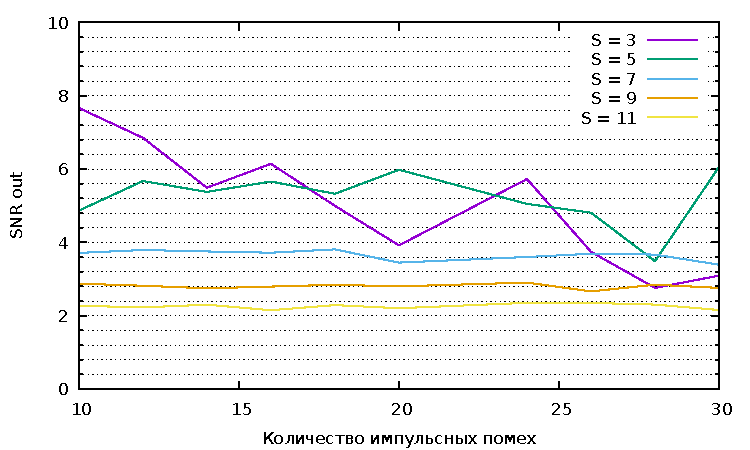
\includegraphics[scale=0.9,page=1]{med.pdf}
			\caption{}
        \end{figure}

\section{Исследование соотношения SNR для линейного усредняющего фильтра}
        \begin{table}[H]
            \centering
            \begin{tabular} { |c|c| }
                \hline
					\textbf{N} & \textbf{$SNR_{out}$} \\ \hline
                    10 & 0.7927 \\ \hline
                    12 & 0.782 \\ \hline
                    14 & 0.822 \\ \hline
                    16 & 0.802 \\ \hline
                    18 & 0.828 \\ \hline
                    20 & 0.821 \\ \hline
                    22 & 0.7948 \\ \hline
                    24 & 0.8321 \\ \hline
                    26 & 0.78 \\ \hline
                    28 & 0.735 \\ \hline
                    30 & 0.761 \\ \hline
            \end{tabular}
        \end{table}

        \begin{figure}[H]
            \centering
            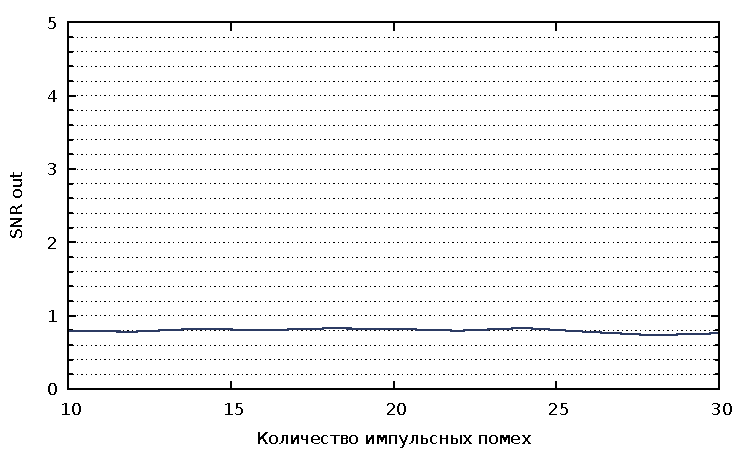
\includegraphics[scale=0.9,page=1]{lin.pdf}
			\caption{Соотношение $SNR_{out}$ на выходе для линейного усредняющего фильтра}
        \end{figure}

\section*{Исследование зависимости SNR от частоты полезного сигнала для фиксированного числа импульсных помех}
        \begin{table}[H]
            \centering
            \begin{tabular} { |c|c| }
                \hline
					\textbf{$F_s$} & \textbf{$SNR_{out}$} \\ \hline
					1  &  34.24 \\ \hline
					4  &  8.4622 \\ \hline
					8  &  4.1745 \\ \hline
					12 &  2.839 \\ \hline
					16 &  2.112 \\ \hline
					20 &  1.75 \\ \hline
					24 &  1.49 \\ \hline
					28 &  1.24 \\ \hline
					30 &  1.171 \\ \hline
            \end{tabular}
            \begin{tabular} { |c|c| }
                \hline
					\textbf{$F_s$} & \textbf{$SNR_{out}$} \\ \hline
					1  &  34.302 \\ \hline
					4  &  8.38 \\ \hline
					8  &  4.19 \\ \hline
					12 &  2.851 \\ \hline
					16 &  2.253 \\ \hline
					20 &  1.74 \\ \hline
					24 &  1.4763 \\ \hline
					28 &  1.2254 \\ \hline
					30 &  1.1561 \\ \hline
            \end{tabular}
            \begin{tabular} { |c|c| }
                \hline
					\textbf{$F_s$} & \textbf{$SNR_{out}$} \\ \hline
					1  &  0.7867 \\ \hline
					4  &  0.765 \\ \hline
					8  &  0.8945 \\ \hline
					12 &  0.801 \\ \hline
					16 &  0.812 \\ \hline
					20 &  0.842 \\ \hline
					24 &  0.7466 \\ \hline
					28 &  0.841 \\ \hline
					30 &  0.779 \\ \hline
            \end{tabular}
			\caption{Для значений N = 3, 5, 15 соответственно}
        \end{table}

        \begin{figure}[H]
            \centering
            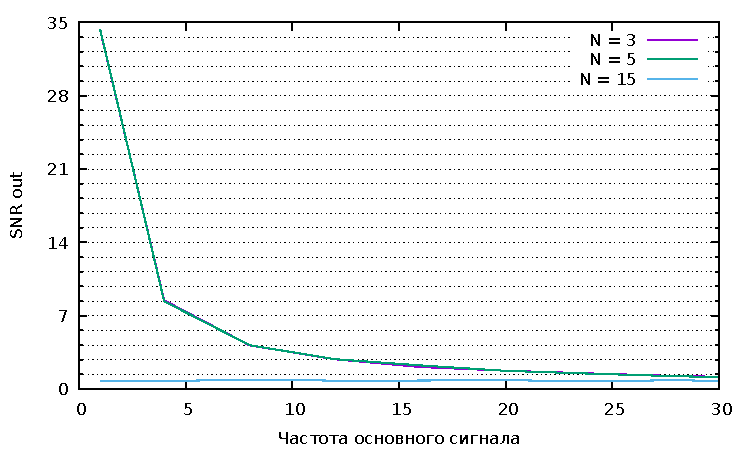
\includegraphics[scale=0.9,page=1]{freq.pdf}
			\caption{Соотношение $SNR_{out}$ на выходе от частоты полезного сигнала $F_s$ для фиксированного числа импульсных помех}
        \end{figure}




\section*{Функциональная схема устройства}
        \begin{figure}[H]
            \centering
            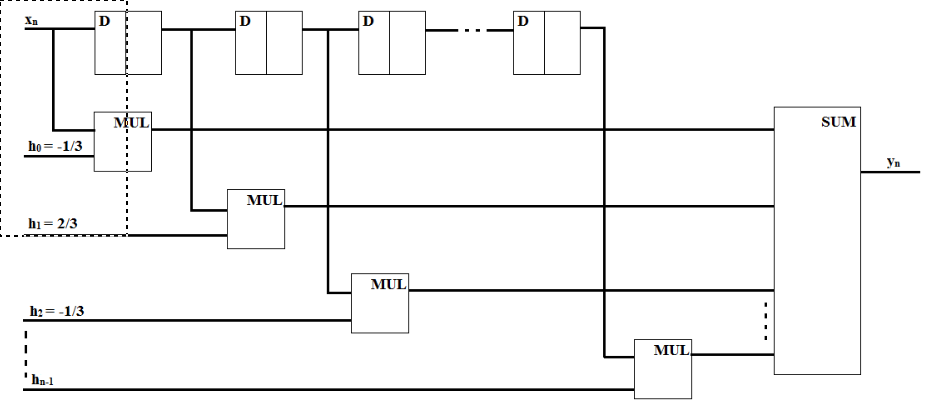
\includegraphics[scale=0.5,page=1]{schema.png}
        \end{figure}

\section*{Вывод}

В результате выполнения лабораторной работы были сделаны следующие выводы.


\end{document}
